\documentclass[11pt]{article}
\usepackage{geometry}                
\geometry{letterpaper}                   
\usepackage{graphicx}
\usepackage{latexsym}
\usepackage{amsmath}
\usepackage{amssymb}
\usepackage{tikz}
\usetikzlibrary{bayesnet}



\title{How to use tikzlibrarybayesnet}

\begin{document}
\maketitle


\begin{figure}[h]\centering
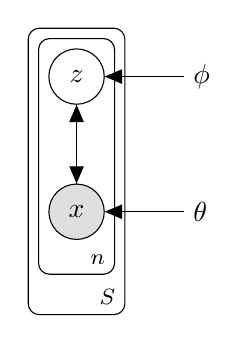
\begin{tikzpicture}
    % Define nodes
    \node[obs]						(x)		{$ x $};
    \node[right = of x]					(theta)		{$\theta$};
    \node[latent, above = of x]		(z)		{$ z $};
    \node[right = of z]					(phi)		{$\phi$};
    
    % Connect nodes
    \edge{z}{x};
    \edge{theta}{x};
    \edge{phi}{z};
    \edge[dashed, bend right]{x}{z};
    
    % add plates
    \plate {sentence} {(x)(z)} {$ n $};
    \plate {corpus} {(sentence)} {$ S $};
\end{tikzpicture}
\caption{VAE}
\end{figure}


\begin{figure}[h]\centering
\begin{tikzpicture}
    % Define nodes
    \node[obs]						(f)		{$ f $};
    \node[right = of f]					(theta)		{$\theta$};
    \node[latent, above = of f]		(a)		{$ a $};
    \node[cond, left = of f]		(e)		{$ e_0^{m} $};
    \node[cond, above = of e]		(m)		{$ m $};
    
    % Connect nodes
    \edge{e,a}{f};
    \edge{m}{a};
    \edge{theta}{f};
    
    % add plates
    \plate {source-sentence} {(f)(a)} {$ n $};
    \plate {corpus} {(source-sentence) (e) (m)} {$ S $};
\end{tikzpicture}
\caption{IBM1}
\end{figure}

\begin{figure}[h]\centering
\begin{tikzpicture}
    % Define nodes
    \node[obs]						(f)		{$ f $};
    \node[latent, right = of f]					(theta)		{$\theta$};
    \node[const, above = of theta]					(alpha)		{$\alpha$};
    \node[latent, above = of f]		(a)		{$ a $};
    \node[cond, left = of f]		(e)		{$ e_0^{m} $};
    \node[cond, above = of e]		(m)		{$ m $};
    
    % Connect nodes
    \edge{e,a}{f};
    \edge{m}{a};
    \edge{theta}{f};
    \edge{alpha}{theta};
    
    % add plates
    \plate {english-tables} {(theta)} {$v_E$}
    \plate {source-sentence} {(f)(a)} {$ n $};
    \plate {corpus} {(source-sentence) (e) (m)} {$ S $};
\end{tikzpicture}
\caption{Bayesian IBM1}
\end{figure}


\begin{figure}[h]\centering
\begin{tikzpicture}
    % Define nodes
    \node[obs]						(f)		{$ f $};
    \node[below = of f]					(theta)		{$\theta$};
    \node[obs, right = of f]        (fprev) {$f_{\text{prev}}$};
    \node[latent, above = of f]		(a)		{$ a $};
        \node[latent, right = of a]     (c)     {$ c $};
    \node[cond, left = of f]		(e)		{$ e_0^{m} $};
    \node[cond, above = of e]		(m)		{$ m $};
    
    % Connect nodes
    \edge{e,a,fprev}{f};
    \edge{m}{a};
    \edge{theta,c}{f};
    \edge{fprev}{c};
    
    % add plates
    \plate {source-sentence} {(f)(a)(fprev)(c)} {$ n $};
    \plate {corpus} {(source-sentence) (e) (m)} {$ S $};
\end{tikzpicture}
\caption{Collocation IBM1: $c \in \{0, 1\}$}
\end{figure}


\begin{figure}[h]\centering
\begin{tikzpicture}
    % Define nodes
    \node[obs]						(f)		{$ f $};
    \node[below = of f]					(theta)		{$\theta$};
    \node[obs, right = of f]        (fprev) {$f_{\text{prev}}$};
    \node[latent, above = of f]		(a)		{$ a $};
        \node[latent, right = of a]     (c)     {$ c $};
    \node[cond, left = of f]		(e)		{$ e_0^{m} $};
    \node[cond, above = of e]		(m)		{$ m $};
    \node[latent, right = of c]		(z)		{$ z $};
    \node[right = of z]		(ab)		{$ \alpha,\beta $};
    
    % Connect nodes
    \edge{e,a,fprev}{f};
    \edge{m}{a};
    \edge{theta,c}{f};
    \edge{fprev}{c};
    \edge{z}{c};
    \edge{ab}{z}
    
    % add plates
    \plate {source-sentence} {(f)(a)(fprev)(c)} {$ n $};
    \plate {corpus} {(source-sentence) (e) (m)} {$ S $};
    \plate {berparams} {(z)} {$v_F$};
\end{tikzpicture}
\caption{Bayesian Collocation IBM1}
\end{figure}



\begin{figure}[h]\centering
\begin{tikzpicture}
    % Define nodes
    \node[obs]						(f)		{$ f $};
    \node[below = of f]					(theta)		{$\theta$};
    \node[obs, right = of f]        (fprev) {$f_{\text{prev}}$};
    \node[latent, above = of f]		(a)		{$ a $};
        \node[latent, right = of a]     (c)     {$ s $};
    \node[cond, left = of f]		(e)		{$ e_0^{m} $};
    \node[cond, above = of e]		(m)		{$ m $};
    
    % Connect nodes
    \edge{e,a,fprev}{f};
    \edge{m}{a};
    \edge{theta,c}{f};
    \edge{fprev}{c};
    
    % add plates
    \plate {source-sentence} {(f)(a)(fprev)(c)} {$ n $};
    \plate {corpus} {(source-sentence) (e) (m)} {$ S $};
\end{tikzpicture}
\caption{Latent gate IBM1: $s \in [0, 1]$}
\end{figure}


\end{document}  
